
\documentclass[a4paper,12pt,single,pdftex]{scrartcl}
%\usepackage[ngerman]{babel}
\usepackage{color}
\usepackage{amsmath}
\usepackage{times}
\usepackage{graphicx}
\usepackage{fancyheadings}
\usepackage{hyperref}
\setlength{\parindent}{0.6pt}
\setlength{\parskip}{0.6pt}
\title{Stats Basics}
 

\begin{document} 
\maketitle
\newpage
%\tableofcontents
\newpage

\section{Tests}
\subsection{Chi-squared test}


Purpose\section{Odds}
 \frac{Happening}{Not \; Happening}

\subsection{Odds of head when flipping a fair coin is 1:1}


Compared to 50\% probability (Odds \# Probs)\subsection{Odds Ratio}
\subsubsection{Ratio of 2 odds}
\par \textbf{
    
  }
\par \textbf{Similar to R-squared, see if X is a good predictor for Y, when compared to not(X). Relationship between 2 things}
\par \textbf{
    
      Test if the {\bf Odds Ratio} is statistically significant
    \\

  }


Chi-squared test

Fisher's exact test

Wald Test\begin{figure}[htb]
\begin{center}
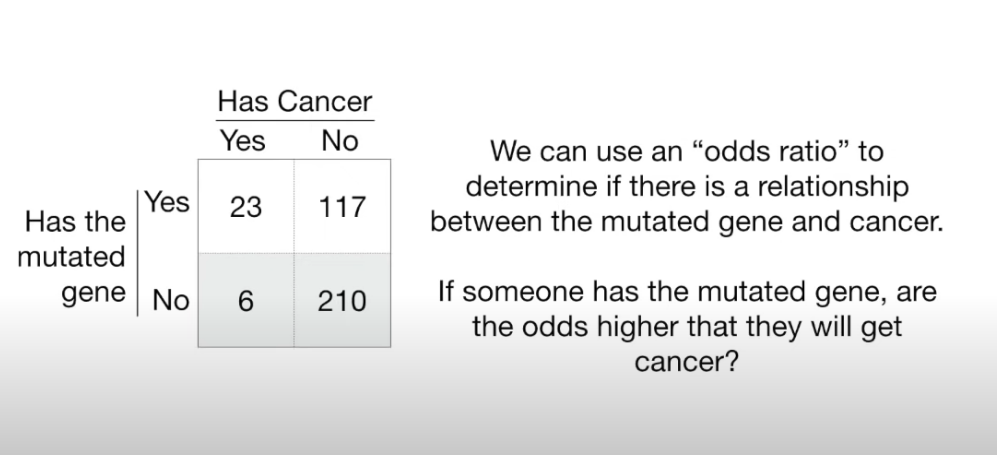
\includegraphics[width=12cm]{Stats_files/png_8965889282046282502}
\caption{Example from Youtube}
\end{center}
\end{figure}


\end{document}
